\section{Global Scoring Functions}

\label{sec4p5}

%{Fig2 page10 is intended as a running example: We show how $s_{FSB}$ behaves on Fig2 (page10-11). Page12 (Fig4 and above), we explain how SAS computes the same case and compares with FSB. We will add explicit references to the case $c<0,d<0$ leading to $s_{FSB}=\frac{cd}{4}$, which corresponds in Figure4 to either case	
%	(b) $\Delta(\hat{b})=\Delta(b)<\frac{c}{2}$ leading to $s_{SAS}=d\Delta(b)<\frac{cd}{2}$ or
%	(c) $\Delta(\hat{b})=0$ leading to $s_{SAS}=0$.}

To select nodes $X$ for pMILP$_X$, we first adapt from the BaB-SR \cite{BaB} and FSB \cite{FSB} functions, %(replacing the symbols from the original paper with those used in our paper.)
 which originally iteratively select one node to branch on for BaB.
 Intuitively, we extract the scoring $s_{SR}$ and $s_{FSB}$ from both BaB-SR and FSB, as the 
 BaB bounding step is not adapted for pMILP. 
 We will call such functions {\em  global scoring} (GS) functions. 
  
 
 They both work by backpropagating gradients vectors $\bm{\lambda}$ from the neurons under consideration in layer $n$, back to neurons to be potentially selected. To do so, they consider the rate of $\ReLU(\bm{u}_k)$ to be 
$r(\bm{u}_k)=\frac{\max(0,\UB(\bm{u}_k))}{\max(0,\UB(\bm{u}_k))-\min(0,\LB(\bm{u}_k))} \in [0,1]$, 
with $r(b)=0$ iff $\UB(b)\leq 0$ and $r(b)=1$ iff $\LB(b)\geq 0$.

\begin{align}
\bm{\lambda}_{n-1} = -{(\bm{W}^n)}^T\bm{1}, \hspace*{4ex}  	\bm{\lambda}_{k-1} = {(\bm{W}^k)}^T\big( r(\bm{u}_k) \odot\bm{\lambda}_{k}\big) \hspace*{4ex}  k\in [n-1,2]
\end{align}


Then, the scoring functions $\bm{s}_{SR}$ and $\bm{s}_{FSB}$ for ReLUs in layer $k$ are computed by approximating how each node would impact the neurons in layer $n$, using the computed $\bm{\lambda}$, differeing only in how they handle the bias $\bm{b}_k$:




\begin{align*}
	\bm{s}_{SR}(k) =& %\bm{1}_{\bm{u}_k>0,\bm{l}_k<0} \odot
	\Biggl\lvert r(\bm{u}_k) \odot \LB(\bm{u}_k) \odot \max(\bm{\lambda}_{k},0)
	+ \max\{0,\bm{\lambda}_{k}\odot\bm{b}_{k}\}-r(\bm{u}_k) \odot\bm{\lambda}_{k}\odot\bm{{b}}_{k}
	\Biggr\rvert  \\
	\bm{s}_{FSB}(k) =& \Biggl\lvert r(\bm{u}_k) \odot \LB(\bm{u}_k) \odot \max(\bm{\lambda}_{k},0)
	+ \min\{0,\bm{\lambda}_{k}\odot\bm{b}_{k}\}-r(\bm{u}_k) \odot\bm{\lambda}_{k}\odot\bm{{b}}_{k}
	\Biggr\rvert
\end{align*}











	
	%In case where the bias is 0, then there is no difference between $s_{SR}$ and $s_{FSB}$.
	Then, ReLU are ranked using these scores, to select the most important unstable ReLUs
	(with $\LB(u_k) < 0 < \UB(u_k)$).
	% as stable ReLUs are linear, thus they are already treated correctly.
	


	
\noindent {\em Running Example:} Consider Fig. \ref{img:FSB_example}. 
It has no bias, so $s_{SR}=s_{FSB}$. We have $\lambda(b)=d$, $\lambda(a)=\frac{cd}{2}$.
The value of $s_{FSB}(a)$ depends on the signs of $c,d$.

We perform a novel comparison between $s_{FSB}(a)$ and $\Delta(z)$, the difference on the {\em maximal bound} computed by pMILP$_X(z)$ when opening the $\ReLU$ of node $a$ ($X=\{a\}$), yielding $\val(\hat{a}) = \ReLU(\val(a))$, versus having $X=\emptyset$, for which 
$\val(\hat{a})$ can be any value in the triangle approximation (Prop. \ref{LP}).
%, Fig. \ref{triangle})).


The most favorable cases are $c < 0 < d$ and $d < 0 < c$: 
as $cd <0$, we have $s_{FSB}(a)=\max(0,\frac{cd}{4}) = 0$.
Because $cd <0$, both $a$ and $\hat{a}$ need to be minimized by MILP$_X$ in order to maximize the value of $z$. For $X=\emptyset$, the LP approximation (=MILP$_\emptyset$) will thus 
set $\val(\hat{a}) = \ReLU(\val(a))$ as this is the minimum value in the triangle approximation. Notice that opening $X=\{a\}$ yields the same $\val(\hat{a}) = \ReLU(\val(a))$.
That is, opening node $a$ is not improving the bound $\UB(z)$, as correctly predicted by the score $s_{FSB}(a)= \Delta(a) = 0$.






\iffalse
\begin{figure}[t!]
	\begin{centering}
	\begin{tikzpicture}[scale=1, >=stealth]
		
		% Draw axes
		\draw[->] (-5,0) -- (4,0) node[right] {$a$};
		\draw[->] (0,-1) -- (0,3) node[above] {$\hat{a}$};
		
		% Draw ReLU function
		\draw[line width=0.4mm, blue] (-3,0) -- (0,0);
		\draw[thick, blue] (0,0) -- (2.5,2.5) node[below, shift={(-1.1,-1.9)}] {$\hat{a} = \ReLU(a)$};
		\draw[thick, blue] (-3,0) -- (2.5,2.5) node[above, shift={(-5.7,-2)}] {$\hat{a} = r(a) (a-\LB)$};
		
		% Add labels
		\draw[dashed] (2.5,0) -- (2.5,2.5) -- (0,2.5); % Optional grid
		\node[below left] at (0,0) {$0$};
		
		% Add tick marks
		
		\foreach \x in {2.5}
		\draw[shift={(\x,0)}] (0,0.1) -- (0,-0.1) node[below] {$\UB$};
		\foreach \x in {-3}
		\draw[shift={(\x,0)}] (0,0.1) -- (0,-0.1) node[below] {$\LB$};
	
		\foreach \y in {2.5}
		\draw[shift={(0,\y)}] (0.1,0) -- (-0.1,0) node[left] {$\UB$};
		
		
	\end{tikzpicture}
		\caption{Triangle approximation with $r(a)=\frac{1}{2}$
		\vspace{-0.3cm}}
	\label{triangle}
	\end{centering}
	\end{figure}
\fi




Case $c>0,d>0$: we have $s_{FSB}(a)=\frac{cd}{4}$.
The value of $a,\hat{a},b,\hat{b}$ should be maximized to maximize the value of $z$, because $W_{bz}=d>0$ and $W_{ab}=c>0$. 
%Each variation of $b$ by $\Delta(b)$ will have an impact $r(b) \cdot \Delta(b)=\frac{\Delta(b)}{2}$ on the value of $\hat{b}$, and thus $\frac{d \Delta(b)}{2}$ on $z$. 
Now, let us call $val(a)$ the maximum value for $a$ 
(same for MILP$_\emptyset$ and MILP$_{\{a\}}$).
The maximum value for $\hat{a}$ under LP ($X=\emptyset$) is 
$\frac{1}{2} \cdot (\val(a)-LB(a))$ following the triangle approximation. 
Now, if $X=\{a\}$, then the value of $\hat{a}$ is $\ReLU(\val(a))$: the difference 
$\Delta(\hat{a})$ is between 0 (for $\val(a)\in \{LB,UB\}$) and $\frac{1}{2}$ (for $\val(a)=0$). The difference $\Delta(b)$ for the value of $b$ is thus between 0 and $\frac{c}{2}$, which means $\Delta(\hat{b}) \in [0, \frac{c}{4}]$, using the upper function of the triangle approximation of rate $r(b)=\frac{1}{2}$, as the value of $\hat{b}$ should be maximized.
This means a difference $\Delta(z) \in [0, \frac{cd}{4}]$ 
(depending on the maximal value $val(a)$), to compare with the fixed 
$s_{FSB}(a)=\frac{cd}{4}$.


\begin{figure}[t!]
	\centering
	\begin{tikzpicture}
		
		\node (input1) {};
		
		%\node (input2) at ($(input1) + (0,-1.5)$) {$n'$};
		
		% Hidden layers
		
		\node (hidden10) at ($(input1) + (2,0.6)$) {$[-1,1]$};
		
		\node (hidden20) at ($(input1) + (2.5,-1.5-0.6)$) {};
		
		\node (hidden50) at ($(input1) + (7.5,0.6)$) {$[-1,1]$};
		
		\node (hidden60) at ($(input1) + (7.5,-1.5-0.6)$) {};
		
		
		\node[circle, draw= black, thick, minimum width = 20,
		minimum height = 20] (hidden1) at ($(input1) + (2,0)$) {$a$};
		%\node[circle, draw= black, thick] (hidden2) at ($(input1) + (2.5,-1.5)$) {$a'$};
		
		\node[circle, draw= black, thick, minimum width = 20,
		minimum height = 20] (hidden3) at ($(input1) + (5,0)$){$\hat{a}$};
		\node (hidden4) at ($(input1) + (5.5,-1)$) {};
		
		
		\node[circle, draw= black, thick, minimum width = 20,
		minimum height = 20] (hidden5) at ($(input1) + (7.5,0)$){$b$};
		%\node[circle, draw= black, thick] (hidden6) at ($(input1) + (7.5,-1.5)$) {$b'$};
		
		
		
		
		% Output layer
		\node[circle, draw= black, thick, minimum width = 20,
		minimum height = 20] (output1) at ($(input1) + (10,0)$){$\hat{b}$};
		
		\node (output2) at ($(input1) + (10.5,-1)$){};
		
			\node[circle, draw= black, thick, minimum width = 20,
		minimum height = 20] (output3) at ($(input1) + (12.5,0)$){$z$};
		
		
		% Connections
		
		%\draw[->,thick] ($(input1) + (-1.5,0)$) -- (input1) node[midway, above] {$[-1,1]$};
		
		% \draw[->,thick] ($(input1) + (-1.5,-1.5)$) -- (input2) node[midway, above] {$[-1,1]$};
		
		\draw[->,thick] (input1) -- (hidden1) node[midway, above] {};
		%\draw[->,thick] (input1) -- (hidden2)node[near start, below] {$-10$};
		
		% \draw[->, thick] (input2) -- (hidden2)node[near start, below] {$0.5$};
		
		
		
		
		
		\draw[->, thick] (hidden1) -- (hidden3) node[midway, above] {open ReLU?};
		%\draw[->, thick] (hidden2) -- (hidden4);
		
		
		
		
		
		\draw[->, thick] (hidden3) -- (hidden5) node[midway, above] {{\color{red}$c$}};			
	
		\draw[->,thick] (hidden4) -- (hidden5)node[near start, above] {};
		%\draw[->,thick] (hidden4) -- (hidden6)node[near start, below] {$1$};
		
		
		\draw[->,thick] (hidden5) -- (output1) node[midway, above] {LP ReLU};
		%\draw[->,thick] (hidden6) -- (output2);
		
		\draw[->,thick] (output1) -- (output3)node[midway, above] {{\color{red}$d$}};
		\draw[->,thick] (output2) -- (output3)node[near start, below] {};
		
		
	\end{tikzpicture}
	\vspace{-0.8cm}
	\caption{A running example with parametric weights {\color{red}$c$} and {\color{red}$d$}}
	\label{img:FSB_example}
\end{figure}



The last case is the most problematic: 
Case $c<0,d<0$, implying that $s_{FSB}(a)=\frac{cd}{4}$, because $cd >0$.
Opening $\ReLU(a)$ will have the same impact on the value of $\hat{a},b$ 
than in case $c>0,d>0$, with $\Delta(b) \in [0,\frac{c}{2}]$.
However, as $d<0$, value of $\hat{b}$ needs to be minimized to maximize the value of $z$. That is, the value of $\hat{b}$ will be the value of $\ReLU(sol(b))$, and the change 
$\Delta(\hat{b})$ will be either 0 in case $\val(b)<0$,
or $\Delta(b) \in [0,\frac{c}{2}]$ for $\val(b)>0$.
That is, $z$ will be modified by either $\Delta(z)=0$ or $\Delta(z) = d \Delta(b)$, to be compared with the fix value $s_{FSB}(a)=\frac{cd}{4}$, which is not always an overapproximation: we have $\Delta(z)=\frac{cd}{2} > s_{FSB}(a)$, 
if $\val(a)=0$ and $\val(b)>0$.

We call {\em global scoring} (GS) these functions $s_{FSB},s_{SR}$  because they score ReLUs as {accurately} as possible, considering that they do not have access to the values 
$\val(a),\val(b)$ maximizing $z$. Following this analysis of $s_{FSB},s_{SR}$, 
next Section presents a novel scoring function more accurate wrt $\Delta(z)$.
	
	
\iffalse
\begin{figure}[t!]
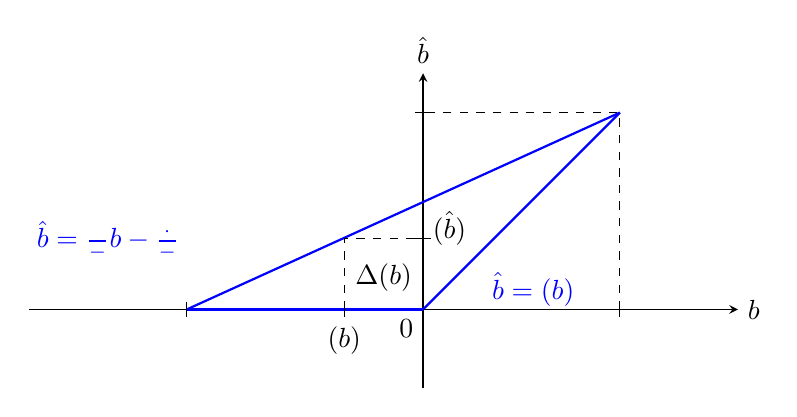
\begin{tikzpicture}[scale=1, >=stealth]
	
	% Draw axes
	\draw[->] (-5,0) -- (4,0) node[right] {$b$};
	\draw[->] (0,-1) -- (0,3) node[above] {$\hat{b}$};
	
	% Draw ReLU function
	\draw[line width=0.4mm, blue] (-3,0) -- (0,0);
	\draw[thick, blue] (0,0) -- (2.5,2.5) node[below, shift={(-1.1,-1.9)}] {$\hat{b} = \ReLU(b)$};
	\draw[thick, blue] (-3,0) -- (2.5,2.5) node[above, shift={(-6.5,-2)}] {$\hat{b} = \frac{\UB}{\UB-\LB} b-\frac{\UB\cdot\LB}{\UB-\LB}$};
	
	% Add labels
	\draw[dashed] (2.5,0) -- (2.5,2.5) -- (0,2.5); % Optional grid
	\node[below left] at (0,0) {$0$};
	
	% Add tick marks
	
	\foreach \x in {2.5}
	\draw[shift={(\x,0)}] (0,0.1) -- (0,-0.1) node[below] {$\UB$};
	\foreach \x in {-3}
	\draw[shift={(\x,0)}] (0,0.1) -- (0,-0.1) node[below] {$\LB$};

	\foreach \y in {2.5}
	\draw[shift={(0,\y)}] (0.1,0) -- (-0.1,0) node[left] {$\UB$};
	
	\draw (-1,0.1) -- (-1,-0.1) node[below] {$\sol(b)$};
	\draw[dashed] (-1,0) -- (-1,0.9) -- (0,0.9);
	\draw (-0.1,0.9) -- (0.1,0.9) node[right, shift={(-0.1,0.13)}] {$\sol(\hat{b})$};
	\node at (-0.5,0.4) {$\Delta(b)$};
	
\end{tikzpicture}
	\caption{}
\label{img:Utility}
\end{figure}
\fi


\iffalse
\subsection*{An example when FSB is not accurate}

See the figure \ref{img:FSB_example}. When the algorithm considers neurons in the layer of $a,a'$, FSB will think $a$ is important, but Utility will think it is not important (Utility value is 0).

Although this example is extreme, similar situations frequently occur in practice.

\subsection*{Comparison on MNIST}

Here we use the network named MNIST $5\times 100$ and a hard image to compare the effect of FSB and Utility function. 

We fix an intermediate bound data for layers before the third hidden layer, and use different methods based on this bound to compute the upper and lower bounds of neurons in the second and third hidden layer.

The plot shows that when only considering neurons in one layer before the target layer, we are significantly better.


\subsection*{Comparison on CIFAR10}

Here we use the network named CNN-B-adv and a hard image to compare the effect of FSB and Utility function. 

We fix an intermediate bound data for layers before the target layers, and use different methods based on this bound to compute the output layer.

The plot shows that our Utility function is significantly better than FSB, and other methods.
\fi
